					\section{Netzwerke}
					\label{chap:Style}


					\definition{Widerstand und Leitwert}

					\beginip
					Der \textbf{Widerstand} bestimmt, wieviel Strom fließen kann, wenn eine bestimmte Spannung angelegt wird. \\
					\begin{center}
						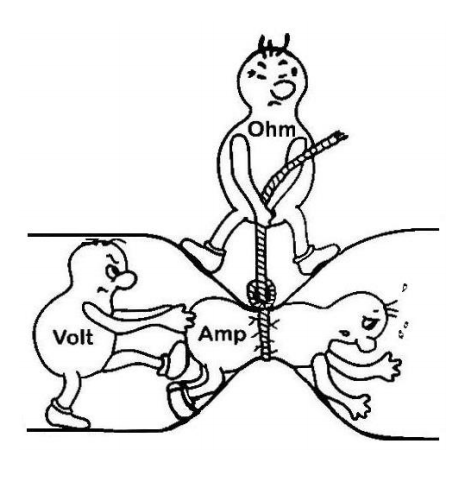
\includegraphics[scale=0.25]{img/widerstand.png}
					\end{center}
					\formulaBegin
					$ R :=  \frac{U}{I} =  \rho  \frac{l}{A}, \ \ \ \ \ \ \  {[R]} = \Omega, Ohm $
					\formulaEnd
					Als \textbf{Leitwert} bezeichnen wir die Inverse des Widerstandes. Er gibt an, wie groß die Spannung ist, wenn ein gewisser Strom fließt. \\
					\formulaBegin
					$ Y = \frac{1}{R} = \frac{A}{\rho \cdot l} $
					\formulaEnd
					\iend




										Da das elektrische Feld wirbelfrei ist, erhalten wir unabhängig vom Weg den gleichen Wert für die Spannung $ U_{AB} $ \\
										Dies bedeutet jedoch auch, dass wir für einen geschlossenen Weg die Spannung $0V$ erhalten müssen, da für jede geschlossene Kurve $\gamma$ gilt:
										\begin{center}
											\vspace{-2mm}

											$\displaystyle \oint_{\gamma} \vec{E} \cdot d\vec{s} = \int_{\gamma_0}^{\gamma_1} \vec{E} \cdot d\vec{s} + \int_{\gamma_1}^{\gamma_0} \vec{E} \cdot d\vec{s} = U_{01} + U_{10} = 0$
										\end{center}
										Mit dieser Erkenntnis können wir die Maschenregel definieren:

										\definition{Maschenregel}
										\beginip
										Die Summe aller Spannungen in einer Masche ergibt $0$ \\
										\formulaBegin
										$\displaystyle \sum_{k=1}^n U_k = 0$
										\formulaEnd

										\iend

										\begin{minipage}{0.6\textwidth}
											\begin{flushright}
											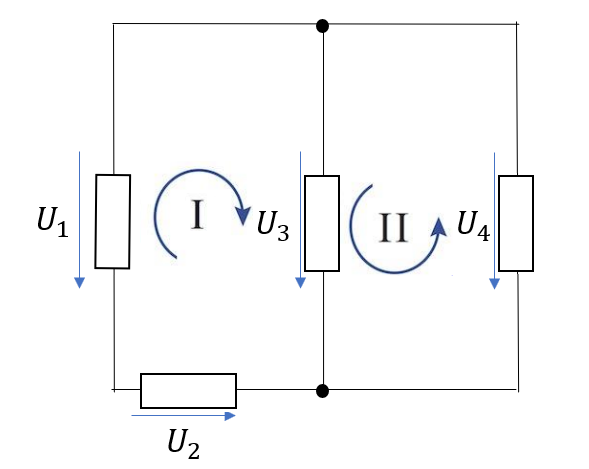
\includegraphics[scale=0.45]{img/maschenregel-2.png}
										\end{flushright}
										\end{minipage}
										\begin{minipage}{0.4\textwidth}
											\textbf{Maschenregel} \\ \\
											I: $\displaystyle (- U_1) + U_3 + (-U_2)  = 0$ \\
											II: $\displaystyle U_3 + (- U_4) = 0 $ \\
											% \vspace{1.5cm}
										\end{minipage}

										Analog können wir mithilfe der Ladungserhaltung argumentieren, dass sämtliche Ladungen, welche in ein Gebiet hineinfließen, auch wieder aus diesem hinausließen müssen.

										\definition{Knotenregel}
										\beginip
										Die Summe aller Ströme die in einen Knoten hinein/hinausfließen muss $0$ ergeben. \\
										\formulaBegin
										$\displaystyle\sum_{i=0}^n I_n = 0 $
										\formulaEnd
					          \iend

										\textbf{Wichtig} Die Knotenregel kann auch auf ein Gebiet von Knoten angewandt werden. \\


										\begin{minipage}{0.6\textwidth}
										\begin{flushright}
												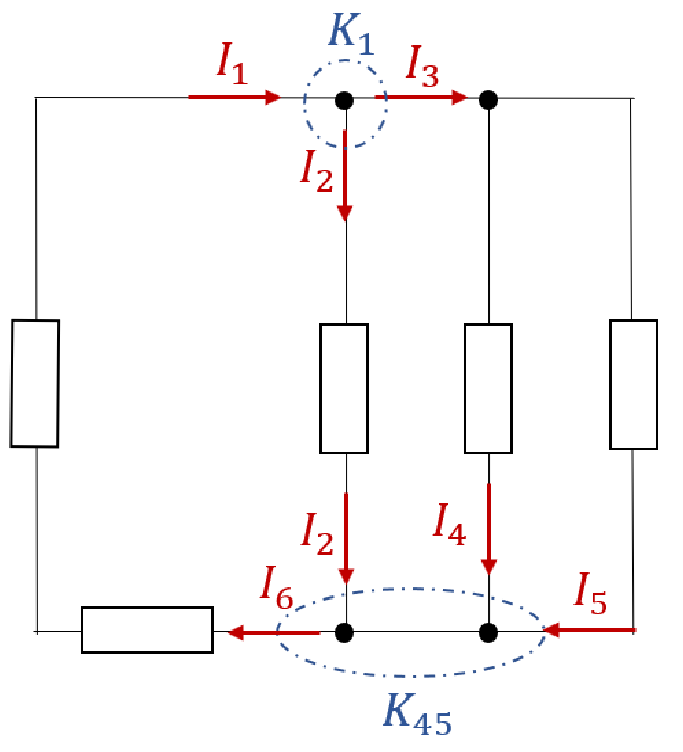
\includegraphics[scale=0.4]{img/knotengl.png}
											\end{flushright}
										\end{minipage}
										\begin{minipage}{0.4\textwidth}

											\textbf{Knotengleichungen} \\ \\
											$\displaystyle K_1$: $ I_1 - I_2 - I_3 = 0 $ \\
											$\displaystyle K_{45}$: $ I_2 + I_4 + I_5 - I_6 = 0 $ \\
										\end{minipage}


					\newpage

										\subsection{Grundlegende Netzwerkumformungen}
										Wir interessieren uns nun dafür, wie sich Widerstände verhalten, wenn wir sie seriell/parallel verknüpfen.
										\definition{Serienschaltung}
										\beginip
										Werden mehrere Widerstände seriell miteinander verbunden, so addieren sich die Widerstandswerte \\
										\formulaBegin
										$\displaystyle R_{serie} = \sum_{i=0}^n R_i = R_1 + R_2 + ...$
										\formulaEnd
										\iend

							        \vspace{1em}

										\textbf{Begründung} \\
										Mehrere Widerstände in Serie können als einen langen Widerstand mit konstanter Fläche angesehen werden. Da die Längenabhängigkeit des Widerstandes im Zähler steht, addieren sich die Werte. \\
										$\displaystyle R_s = \rho \cdot \frac{l_1+l_2}{A} = \rho \cdot \frac{l_1}{A}  + \rho \cdot \frac{l_2}{A}  = R_1 + R_2 $
										\fix
										\begin{center}
											\ibox{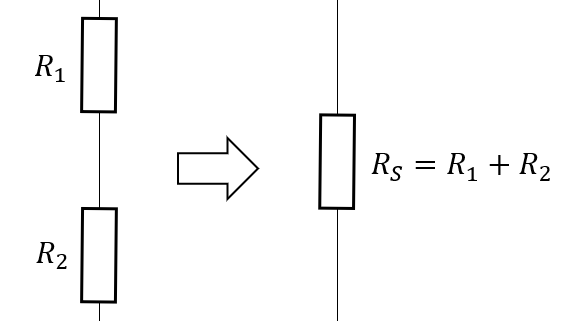
\includegraphics[scale=0.3]{img/serienschaltung.png}}
										\end{center}
					\fix


										\definition{Parallelschaltung}

										\beginip
										Werden mehrere Widerstände parallel miteinander verbunden, so addieren sich die Leitwerte \\
										\formulaBegin
										$\displaystyle Y_{parallel} = \sum_{i=0}^n Y_i \Bigg\rvert$
										$\displaystyle R_{parallel} = \left(\sum_{i=0}^n \frac{1}{R_i}\right)^{-1} = \frac{(R_1 \cdot R_2)}{R_1 + R_2}$
										\formulaEnd
										\iend

					          \vspace{1em}

					          \textbf{Begründung} \\
										Mehrere Widerstände parallel können als einen Widerstand mit größerer Fläche und konstanter Länge angesehen werden. Da die Flächenabhängigkeit des Widerstandes im Nenner steht, addieren sich die Leitwerte. \\
											$\displaystyle Y_p = \frac{1}{\rho} \cdot \frac{A_1 + A_2}{l} = \frac{1}{\rho} \cdot \frac{A_1}{l}  + \frac{1}{\rho} \cdot \frac{A_2}{l}  = Y_1 + Y_2 $


										\begin{center}
											\ibox{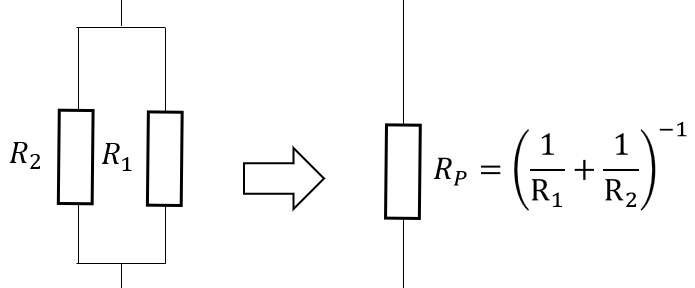
\includegraphics[scale=0.3]{img/parallel.png}}
										\end{center}




										\subsection{Stern Dreieck Umformung}
										Sind Widerstände weder seriell noch parallel geschaltet, sondern sind in einem Stern oder Dreieck angeordnet,
										können folgende Zusammenhänge verwendet werden, um eine Dreieckschaltung in eine Sternschaltung und umgekehrt umzuwandeln.
										\begin{center}
		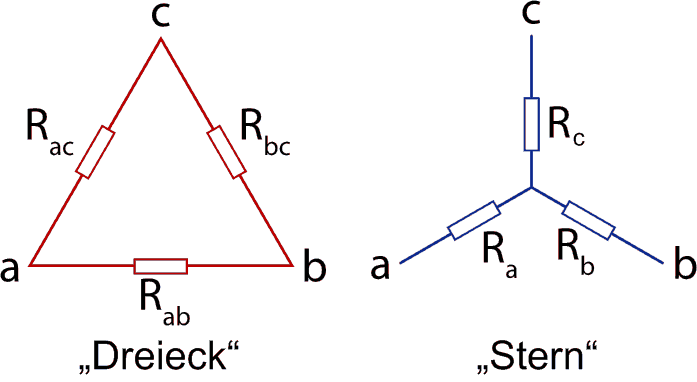
\includegraphics[scale=0.3]{img/Stern-Dreieck-Transformation.png}
\end{center}

\begin{minipage}{0.5\textwidth}
	\begin{center}

	${R}_{AB}=\frac{{R}_{A}{R}_{B}+{R}_{B}{R}_{C}+{R}_{A}{R}_{C}}{{R}_{C}}$\\
	${R}_{AC}=\frac{{R}_{A}{R}_{B}+{R}_{B}{R}_{C}+{R}_{A}{R}_{C}}{{R}_{B}}$\\
	${R}_{BC}=\frac{{R}_{A}{R}_{B}+{R}_{B}{R}_{C}+{R}_{A}{R}_{C}}{{R}_{A}}$\\

	\end{center}
\end{minipage}
\begin{minipage}{0.5\textwidth}
\begin{center}

		${R}_A=\frac{{R}_{AC}{R}_{AB}}{{R}_{AC}+{R}_{AB}+{R}_{BC}}$\\
		${R}_B=\frac{{R}_{AB}{R}_{BC}}{{R}_{AC}+{R}_{AB}+{R}_{BC}}$\\
		${R}_C=\frac{{R}_{AC}{R}_{BC}}{{R}_{AC}+{R}_{AB}+{R}_{BC}}$

	\end{center}
\end{minipage}

\newpage



										\gl{Gleichung}{Spannungsteiler}
										\begingl
										Die Spannungsteilerregel gibt an, wie sich eine Spannung über verschiedene Widerstände aufteilt, wenn diese in \textbf{Serie} geschaltet sind. \\
											\formulaBegin
											$\displaystyle U_{R_x} = U_{ges} \cdot \frac{R_X}{\sum R_i}$
											\\
											2 Widerstände: $
											U_{R_1}  = U_{ges} \cdot \frac{R_1}{R_1 + R_2}$
											\formulaEnd

											\begin{center}
												\ibox{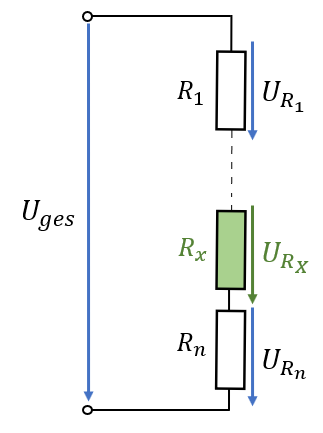
\includegraphics[scale=0.4]{img/spannungsteiler.png}}
											\end{center}
										\iend


										\textbf{Begründung} \\
											Gemäss $\displaystyle U = R \cdot I $ und der Serienschaltung ist der Strom durch alle Widerstände gegeben als $\displaystyle I = \frac{U_{ges}}{\sum R_i} $ \\
											Nun müssen wir nur noch den Strom mit dem gesuchten Widerstand multiplizieren um die Spannung zu erhalten: $\displaystyle U_{R_X} = R_X \cdot I = R_X \frac{U_{ges}}{\sum R_i} $

					\fix
										\gl{Gleichung}{Stromteiler}
										\begingl
											Die Stromteilerregel gibt uns an, wie sich die Ströme in einem Knoten aufteilen, wenn die Widerstände \textbf{parallel} geschaltet sind.
											\fspace
											\formulaBegin
											$\displaystyle I_x = I_{in} \cdot \frac{(R_1 || ... || R_n)} {R_x} $
											\formulaEnd
					\fix
											\begin{center}
												\ibox{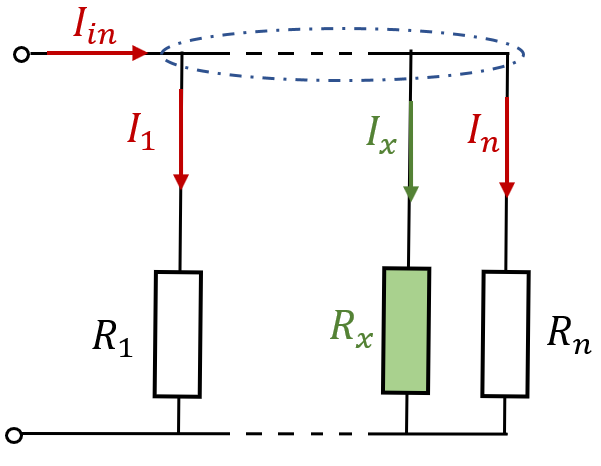
\includegraphics[scale=0.3]{img/stromteiler.png}}
											\end{center}
											\fix
											\textbf{Spezialfall} 2 Widerstände \\
											Falls der Stromteiler nur mit zwei Widerständen angewendet wird, vereinfacht sich die Formel:
											\fspace
											\formulaBegin
											$\displaystyle I_x = I_{in} \cdot \frac{R_y}{R_x + R_y} $
											\formulaEnd
											Der Widerstand, dessen Strom uns \textbf{nicht} interessiert, steht hierbei im Zähler!
										\iend

										\subsection{Grundregeln bei Netzwerkumformungen}
					\fix \fix
										\important{Regel 1}{Expandieren von Knoten}
										\beginip
										 	Knoten können aufgeteilt und mit Verbindungslinien verbunden werden\\
											\begin{center}
											\ibox{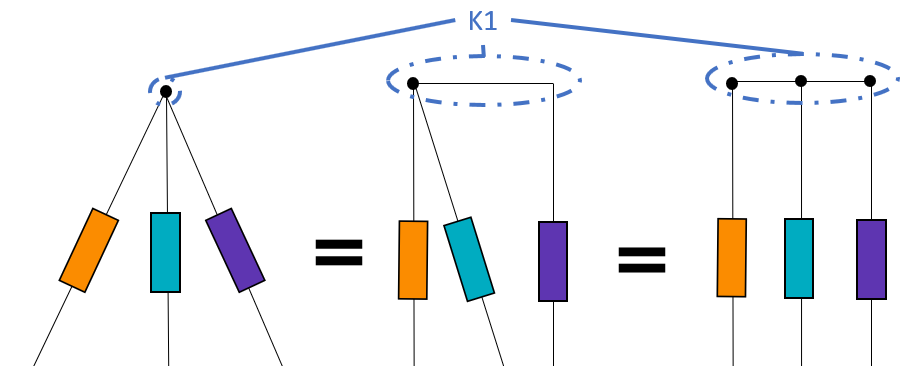
\includegraphics[scale=0.25]{img/knotenexp.png}}
											\end{center}
										\iend

										\fix
					\fix \fix
										\important{Regel 2}{Verschieben von Elementen}
										\beginip
											Elemente können entlang von \textbf{Verbindungslinien ohne Widerständen} verschoben werden\\
											\begin{center}
												\fix \fix \fix
											\ibox{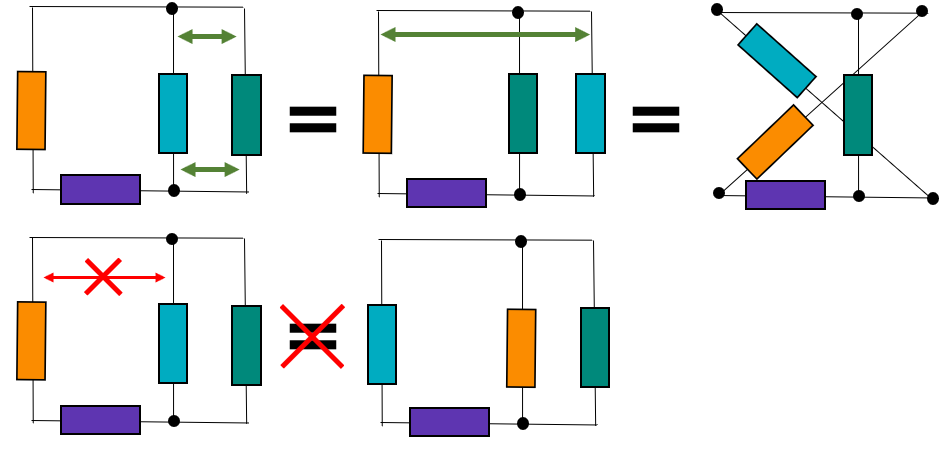
\includegraphics[scale=0.3]{img/verschieben.png}}
											\end{center}
										\iend
					\fix \fix
										\important{Regel 3}{Vertauschen von Elementen in Serie}
										\beginip
											Elemente, die \textbf{in Serie} geschaltet sind, können vertauscht werden
											\begin{center}
												\fix
											\ibox{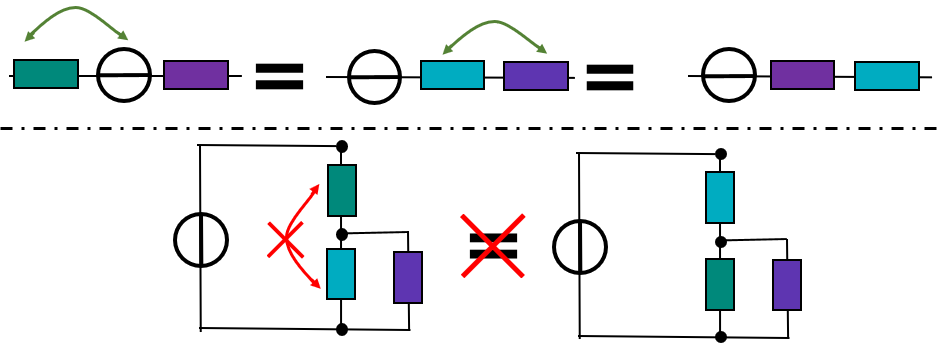
\includegraphics[scale=0.3]{img/vertausch-serie.png}}
											\end{center}
										\iend
					\fix \fix
										\important{Regel 4}{Vertauschen von parallel geschalteten Elementen}
										\beginip
											Elemente die \textbf{parallel} geschaltet sind, können vertauscht werden
											\begin{center}
												\fix
											\ibox{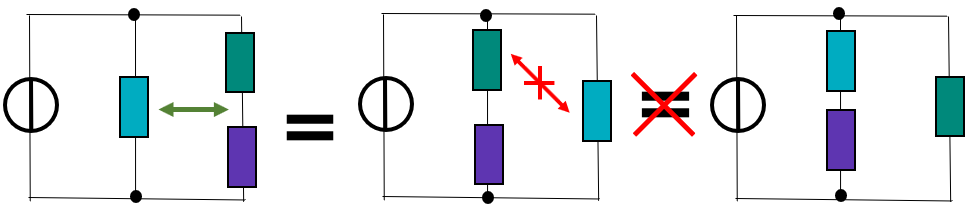
\includegraphics[scale=0.3]{img/vertausch-parallel.png}}
											\end{center}
										\iend
					\fix \fix
										\important{Regel 5}{Knoten kontrahieren}
										\beginip
											(Analog zu 1) Knoten können zusammengezogen werden, sofern sie nicht durch einen Widerstand verbunden sind.
											\begin{center}

											\ibox{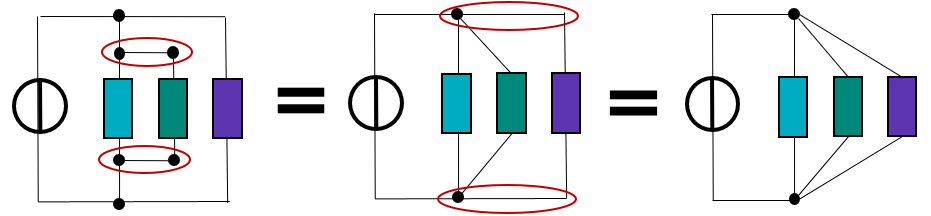
\includegraphics[scale=0.3]{img/knoten-kontrahieren.png}}
											\end{center}
										\iend

										\newpage


										\subsection{Vereinfachungen mithilfe Symmetrieüberlegungen}

										Besitzt ein Netzwerk verschiedene Punkte mit dem selben Potential, so können diese Punkte beliebig verbunden werden.
										Da die Potentialdifferenz immer 0 sein wird, wird niemals Strom zwischen diesen Punkten fliessen.

										\bsptask{Beispiel}{Vereinfachung eines Netzwerkes mit Symmetrie}
										\beginbsp
											Fassen sie alle Widerstände zu einem zusammen unter Verwendung der Symmetrieeigenschaften
											\begin{center}
												%TODO add ppoints
												\ibox{ 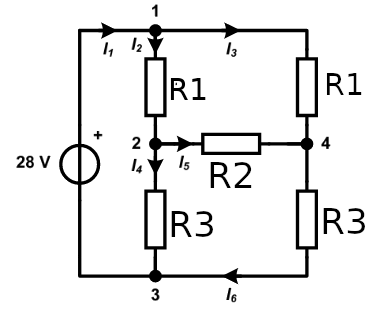
\includegraphics[scale=1.5]{img/sym.png}}
											\end{center}
										\iend

										\bsp{Lösung}{}
										\beginbsp
										Da das Widerstandsnetzwerk symmetrisch bezüglich $R_2$ ist, muss am Punkt 2 und am Punkt 4 das gleiche Potential existieren. \\
										Dies bedeutet, dass über dem Widerstand $R_2$ niemals eine Spannug abfallen und somit auch nie Strom fliessen wird. \\
										\textbf{Lösung 1}: \\
										Wir verbinden die Punkte 2 und 4 mit einem Kurzschluss und erhalten
										\begin{center}
											\ibox{ 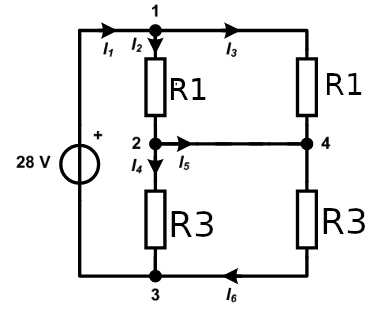
\includegraphics[scale=1]{img/sym-l1.png}}
											$\doubleunderline{R_{ges}} = (R_1 || R_1) + (R_3 || R_3) = \doubleunderline{\frac{1}{2}(R_1 + R_3)}$
										\end{center}

										\textbf{Lösung 2}: \\
										Wir verbinden die Punkte 2 und 4 mit einem Leerlauf und erhalte
										\begin{center}
												\ibox{ 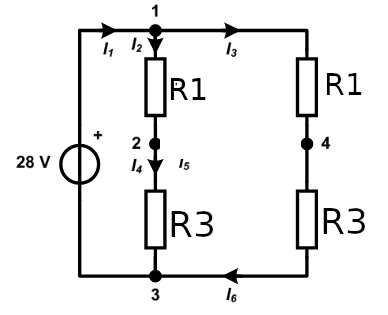
\includegraphics[scale=1]{img/sym-l2.png}}
											$\doubleunderline{R_{ges}} = \big( (R_1 + R_3) || (R_1 + R_3) \big) = \doubleunderline{\frac{1}{2}(R_1 + R_3)}$
										\end{center}


										\iend


\newpage

										\subsection{Vorgehen um Schaltbilder mit einer Quelle zu vereinfachen}
										\begin{enumerate}
											\item Bringe Quelle auf die linke Seite
											\item Forme mit Regel 1 - 5 das Netzwerk soweit um, bis nur noch Spannungs-/Stromteiler oder einfache Maschen vorhanden sind.
											\item Expandiere nun das Netzwerk Schritt für Schritt, bis die Spannung über dem gesuchten Widerstand berechnet werden kann.
										\end{enumerate}

										\bsptask{Beispiel}{}
										\beginbsp
										1) Berechnen Sie $U_x$ in Abhängigkeit des Quellstromes $I$
										\begin{center}
											\fix
										 \ibox{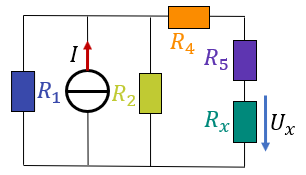
\includegraphics[scale=0.55]{img/aufg1-aufg.png}}
										\end{center}
										\fix
										\iend
										\bsp{Lösung}{}
										\beginbsp
									 \begin{enumerate}
					  				 \item Gemäss Regel 2 können wir $R_1$ und die Stromquelle vertauschen.
										 \item Die Widerstände $R_4 , R_5$ und $ R_x $ können zu $ R_S = R_3 + R_4 + R_5 $ zusammengefasst werden.
										 \item Mithilfe der Stromteilerregel erhalten wir $ I_s = I \cdot \frac{(R_1 || R_2 || R_s)}{R_s} $ und somit $U_s = I \cdot (R_1 || R_2 || R_S) $
										 \item Die Spannung $U_s$ liegt also über dem Widerstand $R_s$ an. Wenn wir diesen wieder in die ursprünglichen 3 Widerstände aufteilen, erhalten wir mithilfe der Spannungsteilerregel $U_x = U_s \cdot \frac{R_x}{R_4 + R_5 + R_x} $
									 \end{enumerate}

										\ibox{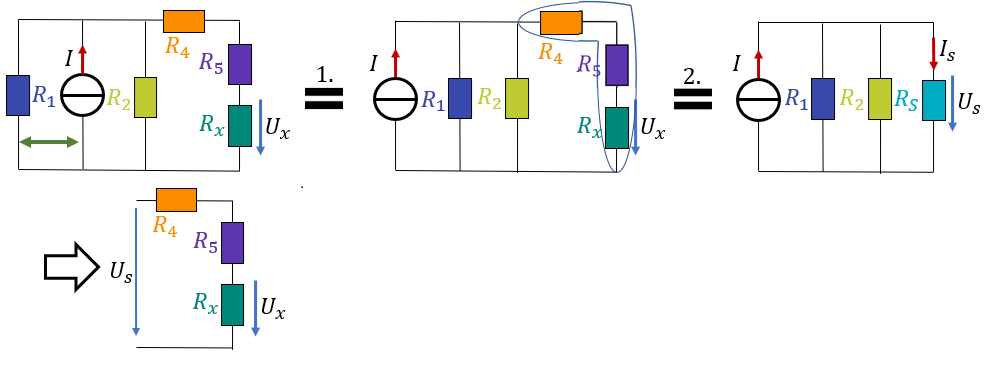
\includegraphics[scale=0.55]{img/bsp1.png}}
										\iend

										In manchen Fällen kann es schwierig sein, die Quelle auf die linke Seite zu bringen oder das Schaltbild nützlich umzuformen. \\
										Um ein erstes Ersatzschaltbild zu erhalten, kann das "Flussverfahren\texttt{"} angewandt werden.

					\newpage
										\bsp{Beispiel}{Flussverfahren}
										\beginbsp
										Beim Flussverfahren überlegt man sich sämtliche Arten, wie der Strom von einem Ende der Quelle zum anderen fliessen kann, und zeichnet somit ein Ersatzschaltbild. \\ \\
										\textbf{Beispiel}
										\begin{center}
											\fix
												\ibox{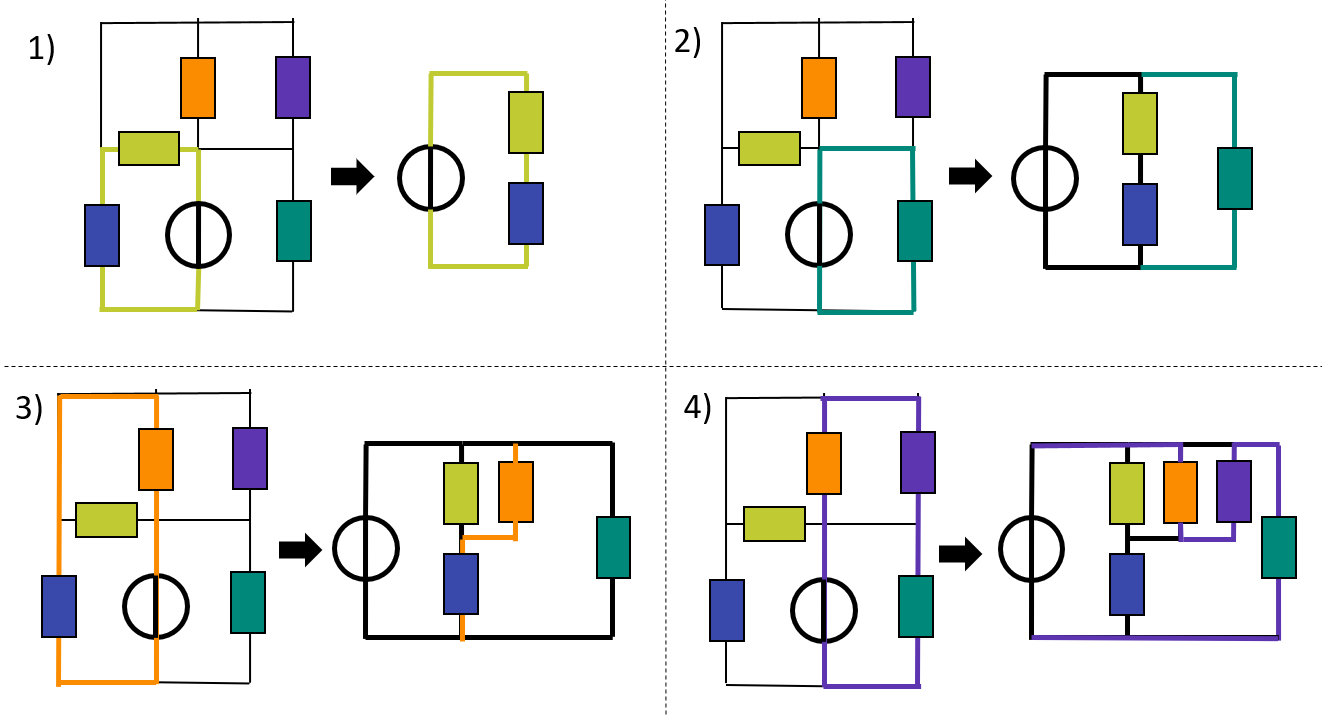
\includegraphics[scale=0.3]{img/fluesse.png}}
										\end{center}
										\iend

										\subsection{Quellen}
										\definition{Ideale Quelle}
										\beginip
										Eine ideale Strom-/Spannungsquelle liefert immer denselben Strom/dieselbe Spannung, unabhängig von der Last, welche angehängt wird.
										\begin{center}
											\ibox{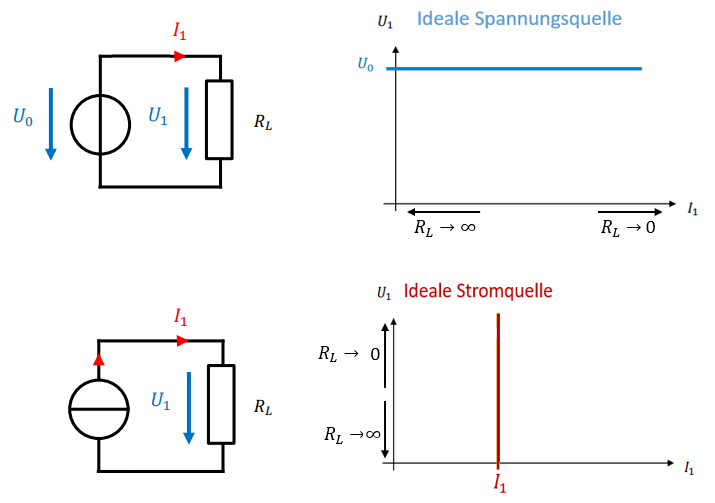
\includegraphics[scale=0.6]{img/ideale_quelle.png}}
										\end{center}

										\iend


										Mit idealen Strom-/Spannungsquellen können wir theoretisch unendlich viel Spannung/Strom über einem Lastwiderstand erzeugen. \\
										(Beispiel ideale Spannungsquelle im Kurzschluss/ideale Stromquelle im Leerlauf) \\
										Bei einer realen Quelle kann jedoch nur eine endliche Spannung/Strom auftreten, wesshalb wir Verluste innerhalb der Quelle mit einem Innenwiderstand $R_i$ modellieren. \\

										\definition{Reale Quelle}
										\beginip
										Eine reale Quelle bezeichnet eine ideale Quelle mit Vorwiderstand. \\
										Bei einer \textbf{Stromquelle} ist der Widerstand \textbf{parallel}, bei einer \textbf{Spannungsquelle} ist der Widerstand in \textbf{Serie}.
											\begin{center}
												\fix
													\ibox{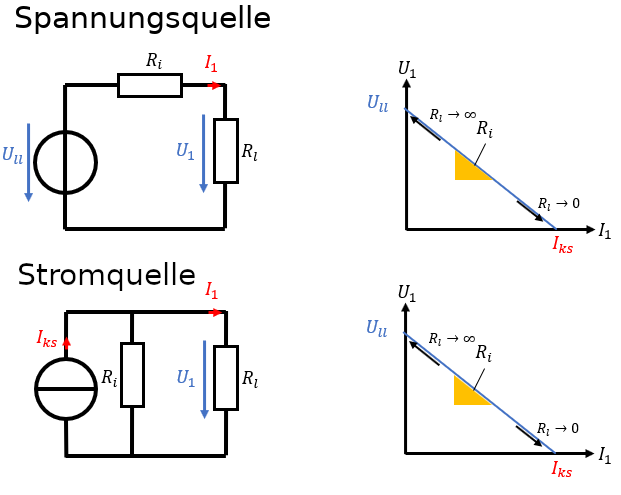
\includegraphics[scale=0.6]{img/realeQuellen.png}}
											\end{center}
										\iend




																				\subsection{Superpositionsprinzip}

																				 Das Superpositionsprinzip besagt, dass wir bei einem Netzwerk mit mehreren Quellen einzelne Teillösungen in Abhängigkeit von nur einer Quelle berechnen und aufsummieren können. \\
																				 Dies gilt jedoch nicht für die Leistung, da diese nicht linear ist! \\
																				 Um das Superpositionsprinzip anzuwenden, müssen wir alle ausser einer Quelle auf \texttt{"}0\texttt{"} setzen. \\
																				 Spannungsquellen werden also mit \textbf{Kurzschlüssen} ersetzt und Stromquellen mit \textbf{Leerläufen}. \\
																				 \begin{center}
																				 	\fix
																				 		\ibox{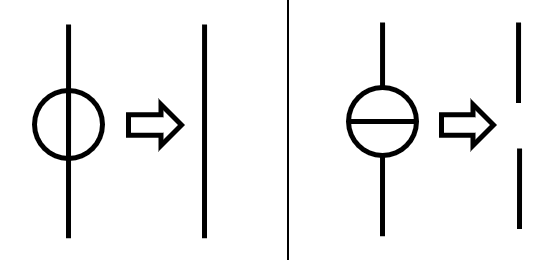
\includegraphics[scale=0.3]{img/superpos-zero.png}}
																				 \end{center}


																				 \textbf{Wieso?} \\
																				 Eine Spannungsquelle zu \texttt{"}0\texttt{"} zu setzen bedeutet, dass über diesem Bauteil keine Spannung abfallen darf. Über einem Kurzschluss wird nie eine Spannung abfallen, da dieser als Widerstand mit Wert 0 modelliert werden kann. \\
																				 Eine Stromquelle zu \texttt{"}0\texttt{"} zu setzen bedeutet, dass durch dieses Bauteil kein Strom fliessen darf. Dies entspricht gerade einem Leerlauf, da dieser als Widerstand mit Wert $\displaystyle \rightarrow \infty$ modelliert werden kann. \\

\newpage


																				 \bsptask{Beispiel}{}
																				 \beginbsp
																				Berechnen Sie die Spannung $U_x$ und die Leistung $P_x$ im folgenden Netzwerk, wenn alle Widerstände $ R = 100 \Omega$ betragen. \\
																					\begin{center}
																						\fix
																					\ibox{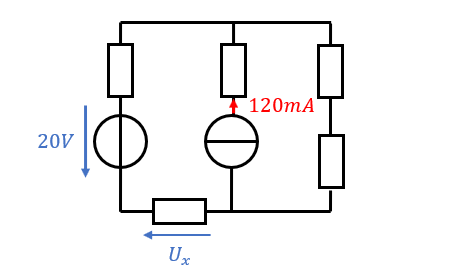
\includegraphics[scale=0.6 ]{img/ex2-1.png}}
																					\end{center}
																					\iend
																					\newpage
																					\bsp{Lösung}{}
																					\beginbsp
																					Zuerst setzen wir die Spannungsquelle zu 0 und erhalten das folgende ESB \\
																					\begin{center}
																						\fix
																					\ibox{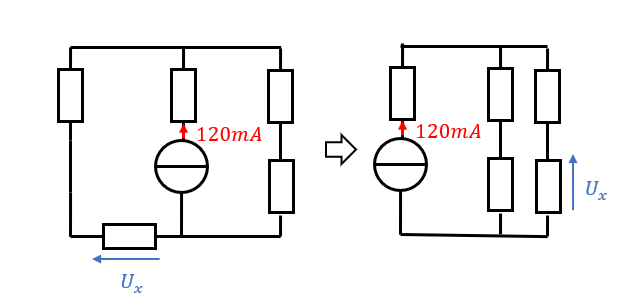
\includegraphics[scale=0.5 ]{img/ex2-2.png}}
																					\end{center}

																					Nun berechnen wir den Strom $I_{x_1}$ durch den Widerstand mithilfe eines Stromteilers: \\
																					$I_{x_1} = 60mA$ \\
																					Die Spannung $U_x$ ist entgegen der Stromrichtung eingezeichnet: \\
																					$U_{x_1} = - R_x \cdot I_x = - 100 \cdot 60mA = -6V $ \\
																					\\
																					Nun setzen wir die Stromquelle zu 0: \\
																					\begin{center}
																						\fix
																					\ibox{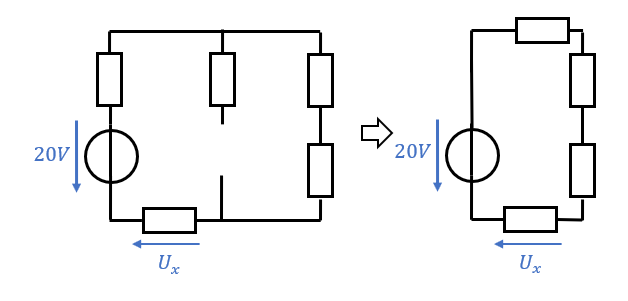
\includegraphics[scale=0.5 ]{img/ex2-3.png}}
																					\end{center}

																					Die Spannung $U_{x_2}$ berechnet sich als Spannungsteiler: \\
																					$U_{x_2} = 20V \cdot \frac{100\Omega}{400\Omega} = 5V$ , $ I_{x_2} = \frac{5V}{100\Omega} = 50mA $\\
																					\\
																					\\
																					\textbf{Superposition:} \\
																					Schlussendlich berechnet sich die Spannung als Summe der Teilspannungen: \\
																					$\displaystyle U_x = U_{x_1} + U_{x_2} = 5V -6V = -1V $ \\
																					Und die Leistung: \\
																					$\displaystyle P_x = \frac{{U_x}^2}{R_x} = 10mW$ \\
																					Welche \textbf{nicht} der Summe der Teilleistungen entspricht: \\
																					$\displaystyle P_{sum} = P_1 + P_2 = U_{x_1} \cdot I_{x_1} + U_{x_2} \cdot I_{x_2} = 360mW + 250mW = 610mW$


																				 \iend

																				 \newpage

																				\subsection{Ersatzquelllen}


																				\definition{Thévenin / Norton Äquivalent}
																				\beginip
																				Jedes Netzwerk mit \textbf{linearen} Bauelementen und 2 Klemmen lässt sich als reale Quelle darstellen. \\
																				\textbf{Thévenin Äquivalent} Darstellung als reale \textbf{Spannungsquelle} mit Leerlaufspannung, die an den Klemmen auftritt \\
																				\textbf{Norton Äquivalent} Darstellung als reale \textbf{Stromquelle}  mit Kurzschlussstrom, der an den Klemmen auftritt\\
																				Der Innenwiderstand entspricht dem von außen gemessenen Widerstand, wenn alle Quellen zu 0 gesetzt werden.
																				\begin{center}
																					\fix
																						\ibox{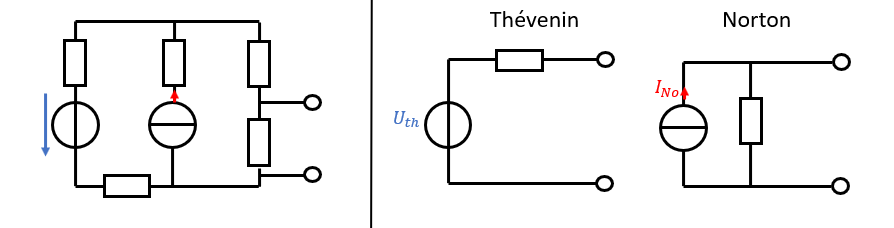
\includegraphics[scale=0.6]{img/nort_the.png}}
																				\end{center}
																				\iend


																				\newpage
																				\vorgehen{Vorgehen}{Ersatzquelle für gegebenes Schaltbild mit offenen Klemmen finden}
																				\beginvor
																				\begin{itemize}

																				  \item[1.] Betrachte die Schaltung. Sind mehr Stromquellen vorhanden, so ist es häufig einfacher den Kurzschlussstrom zu berechnen. Bei mehr Spannungsquellen die Leerlaufsspannung. \\
																				  Wiederhole folgendes für alle Quellen $i$: \\
																				  \end{itemize}
																				  \beginip
																				  \begin{itemize}

																				  \item [2.  ]  Setze alle Strom / Spannungsquellen ausser einer zu 0. (Stromquelle $\rightarrow$ Leerlauf, Spannungsquelle $\rightarrow$ Kurzschluss)
																				  \item[3. ] Versuche die einzelne Quelle auf die linke Seite zu bekommen. (Siehe Skript \texttt{"}Flussverfahren\texttt{"})
																				  \item[4.a)] \textbf{Kurzschlussstrom}
																				  \begin{enumerate}
																				  \item Schliesse die Klemmen kurz und bezeichne den Strom, welcher durch diese Klemmen fliesst als $I_{ks}^{(i)}$.
																					%TODO ADD BILDER
																				  \item Versuche mittels Stromteilern den gesuchten Strom zu berechnen. Falls eine direkte Verbindung von Stromquelle über den Kurzschluss zur Quelle zurückfürt, ist der Kurzschlussstrom gleich dem Strom der Quelle (=0 bei Spannungsquelle). \\
																				  Ist die Quelle keine Stromquelle, so kann evt. ein serieller Widerstand verwendet werden, um die Quelle umzuformen.
																				  \end{enumerate}
																				  \item[4.b)] \textbf{Leerlaufspannung}
																				  \begin{enumerate}
																				  \item Zeichne einen Spannungspfeil zwischen den Klemmen und bezeichne die Spannung als $U_{LL}^{(i)}$.
																				  \item Versuche mittels Spannungsteiler die gesuchte Spannung zu berechnen. Falls kein Strom von der Spannungsquelle fliessen kann (Leerlauf unterbricht die komplette Schaltung), so ist die Leerlaufspannung gleich der Spannung der Spannungsquelle (=0 bei Stromquelle). \\
																				  Ist die Quelle keine Spannungsquelle, so kann evt. ein paralleler Widerstand verwendet werden, um die Quelle umzuformen.
																				  \end{enumerate}
																				\end{itemize}

																				  \iend
																				\begin{itemize}

																				  \item[5.] \textbf{Innenwiderstand}
																				  \begin{enumerate}
																				    \item Setze \textbf{alle} Quellen auf 0. Versuche nun die Widerstände solange umzuformen, bis nur noch ein Ersatzwiderstand vorhanden ist. (Ggf. \texttt{"}Flussverfahren\texttt{"} mit offener Klemme anwenden)
																				    \item Bezeichne den Wert des Widerstandes als $R_i$
																				  \end{enumerate}
																				  \item[6.a)] \textbf{Thévenin Äquivalent} Spannungsquelle mit seriellem Innenwiderstand. \\
																				  Werte: $\displaystyle   R= R_i$, $U_q = \sum_i U_{LL}^{(i)} = (\sum_i I_{ks}^{(i)})\cdot R_i$

																				  \item[6.b)] \textbf{Norton Äquivalent} Stromquelle mit parallelem Innenwiderstand. \\
																				  Werte: $\displaystyle  R= R_i$, $I_q = \sum_i I_{ks}^{(i)}) = \frac{\sum_i U_{LL}^{(i)}}{R_i}$

																				  \end{itemize}

																				\iend





																				\newpage
																				\bsptask{Beispiel}{Thévenin Äquivalente Schaltung}
																				\beginbsp
																				Geben Sie eine Thévenin Äquivalente Schaltung (Innenwiderstand $R_i$, $U_{Th}$) für folgende Klemmen an. Alle Widerstände haben Wert $100\Omega$ \\

																				\begin{center}
																					\fix
																						\ibox{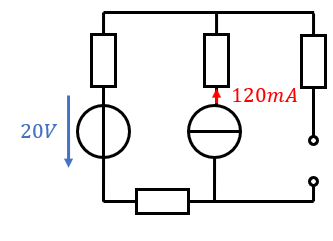
\includegraphics[scale=0.4]{img/ex3-1.png}}
																				\end{center}
																				\iend
																				\bsp{Lösung}{}
																				\beginbsp																				Zuerst berechnen wir die Leerlaufspannung für die Stromquelle: \\
																				$U_{LL_1} = 120mA \cdot 200 \Omega = 24V$ \\
																				Danach die Leerlaufspannung für die Spannungsquelle: \\
																				$ U_{LL_2} = 20V$\\
																				Die Gesamtspannung und somit die Spannung der Ersatzspannungsquelle beträgt: \\
																				$\doubleunderline{U_{Th}} = U_{LL_1} + U_{LL_2} = \doubleunderline{44V}$ \\

																				Nun müssen wir noch den Innenwiderstand berechnen. Dazu setzen wir alle Quellen zu 0 und berechnen den von aussen gemessenen Widerstand:\\
																				\begin{center}
																					\fix
																						\ibox{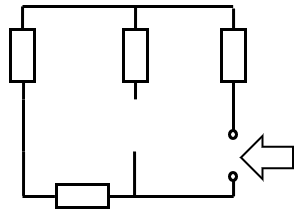
\includegraphics[scale=0.6]{img/ex3-2.png}}
																				\end{center}
																									$\doubleunderline{R_i} = 100\Omega + 100\Omega  + 100\Omega  = \doubleunderline{300 \Omega} $
																				\iend

																				\newpage
										\subsection{Leistungsanpassung}
										\definition{Leistung}
										\beginip
											Als Leistung bezeichnen wir das Produkt von Strom und Spannung. \\
											Sie bezeichnet die in einer Zeitspanne umgesetzte Energie an einem Bauteil. \\
											\formulaBegin
											$\displaystyle P := U \cdot I = \frac{U^2}{R} = I^2 \cdot R $
											\formulaEnd
										\iend

										\definition{Maximale Leistung}
										\beginip
										Um bei einer realen Quelle maximale Leistung an einen Lastwiderstand abzugeben, muss der Lastwiderstand gleich gross sein wie der Innenwiderstand der Quelle. \\
										\formulaBegin
										$ R_i = R_L \Rightarrow P = P_{max}$
										\formulaEnd
										\begin{center}
											\ibox{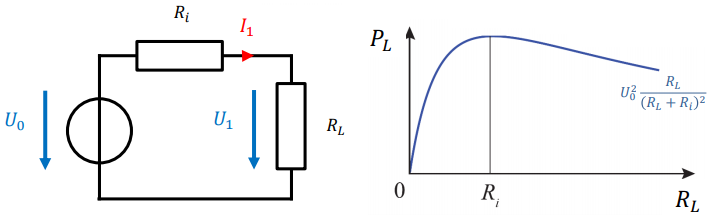
\includegraphics[scale=0.5]{img/leistungsanpassung.png}}
										\end{center}
										\iend
										\textbf{Begründung} \\
										Die Leistung an einem Lastwiderstand in Serie ist gegeben als: \\
										$ \displaystyle P_L = U_L \cdot I_L = \frac{U_L^2}{R_L} = \frac{( U_0 \frac{R_L}{R_L + R_i})^2}{R_L} = U_o^2 \cdot \frac{R_L}{(R_L + R_i)^2}$ \\
										$\displaystyle \frac{d}{dR_L} (P_L) = - U_0^2 \cdot \frac{R_L - R_i}{(R + R_L)^3} = 0 \Rightarrow R_L = R_i  \Rightarrow P_L = P_{max}$





















																														\vorgehen{Vorgehen}{Leistung über einer Last maximieren}
																														\beginvor
\textbf{Falls möglich}
\begin{itemize}
  \item [1. ] Entferne Komponenten über denen die Leistung maximiert werden soll und ersetze sie mit offenen Klemmen (Fasse die entfernten Komponenten als einen Lastwiderstand zusammen).
  \item [2. ] Berechne von den Klemmen den Innenwiderstand.
  \item [3. ] Innenwiderstand $R_i \rightarrow R_L = R_i$
  \item [4. ] Falls maximale Leistung gefragt: Berechne Leerlaufspannung oder den Kurzschlussstrom. $\displaystyle P_{max} = \frac{U_{LL}^2} {4 \cdot R_i } $
\end{itemize}

\textbf{Sonst}

\begin{itemize}
  \item [1. ] Finde einen Ausdruck für $U_L$ und $I_L$
	\item [2. ] Berechne $P = U_L \cdot I_L$
	\item [3. ] Leite $P$ nach dem veränderlichem Widerstand ab und setze zu 0 um ein Maximum zu finden
\end{itemize}


																														\iend
\newpage
\bsptask{Beispiel}{Leistungsanpassung}
\beginbsp
Berechnen sie für folgendes ESB den Wert für $R_L$ bei dem $R_L$ maximale Leistung aufnimmt.
\begin{center}
	\ibox{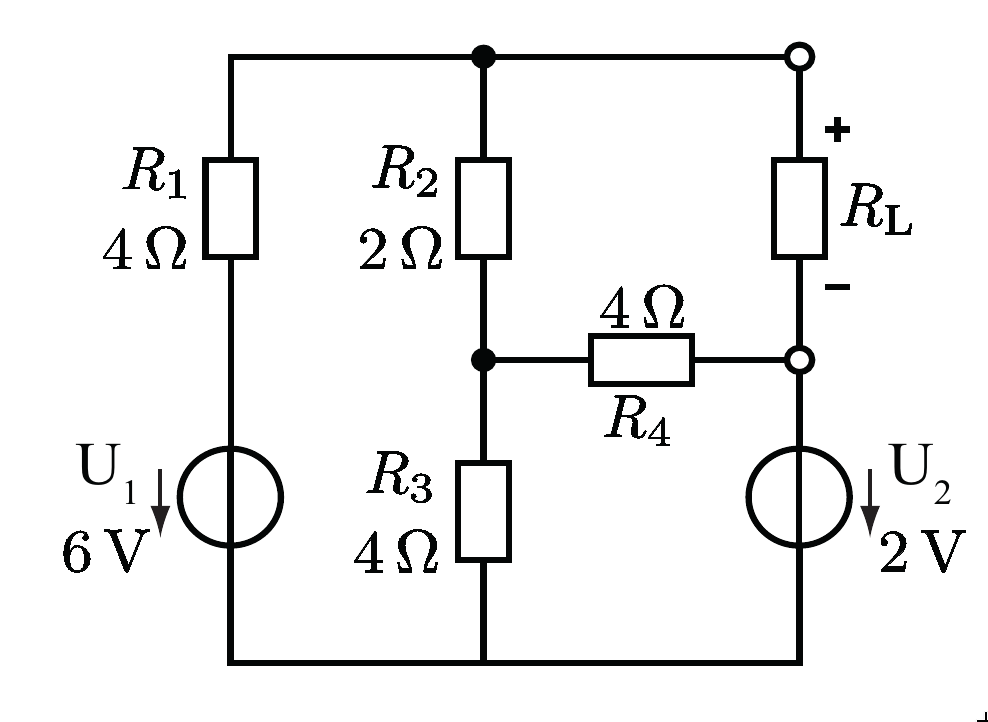
\includegraphics[scale=0.2]{img/leistungsanp.png}}
\end{center}
\iend

\bsp{Lösung}{}
\beginbsp
Um die Leistung über $R_L$ zu maximieren, entfernen wir den Widerstand und berechnen den Innenwiderstand bezüglich den Klemmen. \\
Für die Berechnung des Innenwiderstandes, werden alle Spannungsquellen kurzgeschlossen.
\begin{center}
	\ibox{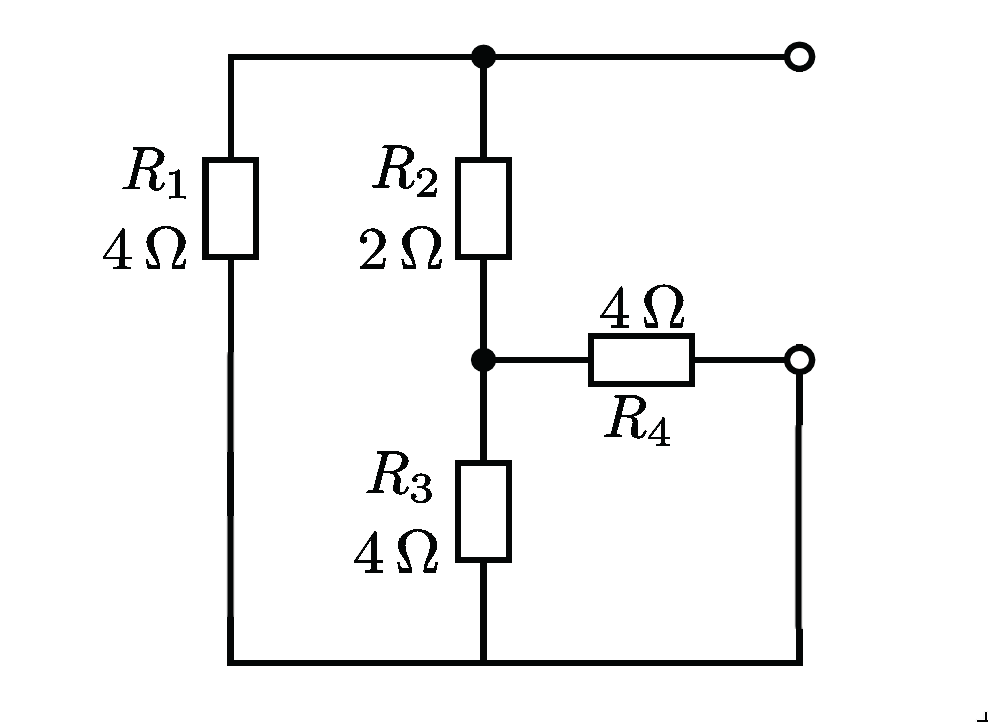
\includegraphics[scale=0.6]{img/leistungsanp_lsg.png}}
\end{center}
Nun müssen nur noch alle Widerstände zu einem zusammengefügt werden:
\begin{center}
	$R_i = (R_1 || R_2 + (R_3 || R_4 )) = 2 \Omega$ \\
	$\doubleunderline{ R_L = R_i = 2 \Omega}$
\end{center}
\iend










										 \newpage





					          \subsection{Analyse umfangreicher Netzwerke}

					           Möchten wir in Netzwerken sehr viele Grössen berechnen, oder ist das Netzwerk sehr komplex, so können andere (meist Computer basierende) Verfahren verwendet. \\
					           Sämtliche Verfahren bauen darauf auf, dass für ein beliebiges Netzwerk das Aufstellen sämtlicher Knoten und Maschengleichungen genügt, um alle gesuchten Grössen zu berechnen. \\

					          \important{Unabhängige Gleichungen}{}
					          \beginip
					             Seien z die Anzahl Zweige eines Netzwerkes (Verbindungen 2-er Knoten) und k die Anzahl Knoten, so müssen z linear unabhängige Gleichungen gefunden werden, um alle Grössen im Netzwerk zu berechnen.  \\Die Gleichungen können folgendermassen gefunden werden: \\
					             \formulaBegin
					              (k-1) Gleichungen können aus Knotengleichungen gefunden werden. \\
					              (z - (k-1)) übrige Gleichungen werden mithilfe von Maschengleichungen gefunden.
					             \formulaEnd
					           \iend


					           \vorgehen{Vorgehen}{Analyse von Umfangreichen Netzwerke}{}
					           \beginip
					            \begin{center}
					              \begin{itemize}
					                \item Entferne alle Widerstände und Quellen und zeichne das Schaltbild neu.
					                \item Nummeriere alle Konten. Die Anzahl der Knoten wird mit k bezeichnet.
					                \item Alle Verbindungslinien, welche zwei Knoten verbinden, werden als Zweige bezeichnet. \#Zweige = z
					                \item Definiere Ströme für jeden Zweig und stelle (k-1) Knotengleichungen auf. Schreibe diese am besten bereits in Matrix schreibweise: \\
					                Bsp: $I_1 + I_2 = I_3, I_3 - I_4 = 2A $: \\
					                $
					 \left[ {\begin{array}{cccc}
					    1 & 1 & -1 & 0 \\
					    0 & 0 & 1 & -1 \\					\end{array} } \right] \left[ {\begin{array}{c} I_1 & I_2 & I_3 & I_4 \\ \end{array} } \right] =   \left[ {\begin{array}{c}  0 & 2A\\ \end{array} } \right] $ \\

					                \item Finde z - (k-1) unabhängige Maschengleichungen. (Mittels vollständiger Baum / Auftrennen der Maschen)
					                \item Ersetze die Spannungen der Maschengleichung mit Strom mal Widerstand und ergänze das Gleichungssystem.
					                \\ Bsp:
					                $U_1 + U_2 = 5V, U_2 - U_3 = U_4$ \\ $ \rightarrow R_1 \cdot I_1 + R_2 \cdot I_2 = 5V, R_2 \cdot I_2 - R_3 \cdot I_3 - R_4 \cdot I_4 = 0$ \\
					                $
					 \left[ {\begin{array}{cccc}
					    1 & 1 & -1 & 0 \\
					    0 & 0 & 1 & -1 \\
					    \mathbf{R_1} & \mathbf{R_2} & 0 & 0 \\
					    0 & \mathbf{R_2} & \mathbf{-R_3} & \mathbf{-R_4} \\
					\end{array} } \right] \left[ {\begin{array}{c} I_1 & I_2 & I_3 & I_4 \\ \end{array} } \right] =   \left[ {\begin{array}{c}  0 & 2A & \mathbf{5V} & \mathbf{0} \\ \end{array} } \right] $ \\

					              \end{itemize}
					            \end{center}
					            \iend
